\documentclass[conference,compsoc]{IEEEtran}

% --- Packages ---

\usepackage{lmodern}
\usepackage{graphicx}
\usepackage{amsmath,amssymb}
\usepackage{booktabs}
\usepackage{listings}
\usepackage{enumitem}
\usepackage{hyperref}
\usepackage{float}
\hypersetup{hidelinks}

% Reduce spacing around sections and subsections
\usepackage{titlesec}
\titlespacing*{\section}{0pt}{8pt plus 2pt minus 2pt}{4pt plus 2pt minus 2pt}
\titlespacing*{\subsection}{0pt}{6pt plus 2pt minus 2pt}{3pt plus 2pt minus 2pt}

% Make section and subsection titles smaller
\titleformat*{\section}{\normalsize\bfseries}
\titleformat*{\subsection}{\small\bfseries}

% --- Document ---
\begin{document}

\title{A Comparative Empirical Study of FIDO2 and Its Predecessors}

\author{
\IEEEauthorblockN{Anderko Máté}
\IEEEauthorblockA{Óbuda University \\ mate.anderko@stud.uni-obuda.hu}
}

\maketitle

\begin{abstract}
The FIDO2 standard, introduced by the FIDO Alliance and the World Wide Web Consortium (W3C) in 2018, it has been hailed as the "Kingslayer of User Authentication".
This paper presents the implementation of a FIDO2 + WebAuthn authentication system and shows an analysis on different user authentication philosophies
The analysis assesses a FIDO2, a 2FA and a password only system on their resistance to common security threats using the STRIDE threat modeling framework and evaluates their performance.
The objective is to determine how adopting FIDO2 influences the security and system resource requirements.
\end{abstract}

\section{Introduction}
Since the dawn of computing the weakest link in most information systems has been the people creating and using them. We choose easy to remember password that might be prone to dictionary attacks, then we overcomplicate them just to forget them, so to only have to remember a couple passwords we reuse them across sites, also we easily fall for social engineering attacks, like phishing. Sufficiently long, unique, and complex passwords with proper rate limiting remain impractical to brute-force, so compromises overwhelmingly exploit human factors and credential leaks rather than cryptographic weakness. 

To mitigate the weaknesses of a password only environment one-time codes (SMS/TOTP) ere introduced, this is 2 or Multi Factor Authentication, which is meant to reduce the risk of falling for credential stuffing attacks and make phishing more complicated. 2FA doesn't address the core issue of legacy authentication though.

FIDO2/WebAuthn addresses the limitations at last by replacing shared secrets with origin-bound public-key cryptography and local user verification (biometrics or a device PIN). Private keys never leave the authenticator, and the server stores only public keys, eliminating password reuse and greatly reducing the value of stolen databases. Because assertions are tied to the requesting origin, generic phishing and OTP-relay attacks fail by design. In practice, passkeys (discoverable credentials) further streamline the flow across platforms using platform sync or roaming security keys.

This paper adopts that progression from passwords to 2FA to FIDO2 
In the coming section we will walk through 
\begin{itemize}
    \item Mapping common vulnerabilities
    \item Implementing a fully passwordless FIDO2 system
    \item Creating a plan for a STRIDE based analysis
    \item Testing the systems for vulnerabilities
    \item Comparing the systems in terms of performance and security.
\end{itemize}

\section{Similar and Related Work}\label{sec:related}

This section reviews research on the security, usability, and adoption of FIDO2, also shows a comparison with this here work.

\subsection{Formal and Theoretical Analyses}
Barbosa and their team \cite{barbosa2021provable} offers a formal model of FIDO2 and, through theoretical analysis, show resistance to credential-phishing and replay attacks. In contrast, the present work examines a deployed FIDO2 stack with STRIDE, emphasizing practical security implications and performance (latency, memory, compute).


\subsection{Empirical and Usability Studies}
Lyastani and their team \cite{lyastani2020kingslayer} created an empirically FIDO2's usability analyses. The study shows significant usability gains and phishing resistance compared to passwords and 2FA. Their work relied on user studies and perception metrics rather than system-level measurements.

Unlike these human-centered, behavioral studies, this work isolates the technical performance and security aspects of FIDO2.

\subsection{Positioning of This Work}
Key contributions:
\begin{enumerate}
    \item Operational implementation of FIDO2/WebAuthn alongside password-only and 2FA baselines.
    \item Structured STRIDE analysis, grounded in Barbosa’s theoretical model.
    \item Empirical performance results—latency, memory footprint, computational load—that complement usability-centric studies (e.g., Lyastani).
\end{enumerate}

Unlike work centered on formal guarantees or user experience, this study examines how adopting FIDO2 shifts real-world security posture and runtime efficiency.




\section{Common Authentication Vulnerabilities}\label{sec:common-vulnerabilities}
Bad actors find the most creative ways to attack authentication systems, these are called attack vectors. The goal of this section is to outline how the vulnerabilities work, which the paper will address in later sections, and also to shine a ligh on why traditional password or even basic MFA schemes struggle against them.s


\subsection{Weak Passwords and Brute-Force Attacks}
Users often choose simple passwords, making them easy targets for brute-force attacks \cite{Ma2022ProspectsPassword}. A simple brute-force attack tries to crack the user's password by trying random character combinations. Rate limiting and sufficient password length makes the attack redundant. A dictionary attack is a more sophisticated version of a brute-force attack, where attackers use common wordlists, lists of frequenly used passwords or they systematically guess combinations to find the password. In the case of brute-force not cryptographic weaknesses, but bad password hygiene and the site's lack of password complexity enforcement leads to the compromise,.


\subsection{Credential Stuffing and Password Reuse}
Credential stuffing exploits password reuse across websites. In the event of a databreach the user's password may get leaked, this creates an opportunity for bad actors, who then use the credentials on other sites to try to gain access to other accounts.\cite{Nisenoff2023PasswordReuse}. The process can be well automated, thus the reuse of credentials turns one breach into many.


\subsection{Social Engineering Attacks}
Many attacks rely on human gullability instead of technical flaws. Phishing, SIM swap, and push fatigue attacks are such attacks.


\subsubsection{Phishing and OTP Relay}
Phishing deceives users into revealing credentials on fake websites, that mimic the working of the site the user is familiar with. Attackers can proxy the login and capture OTP codes in real time, bypassing traditional 2FA, this is commonly referred to as a real-time phishing proxy. OTP capturing is Adversary-in-the-Middle type attack\cite{Kasemodel2025BlueTOTP}.

\subsubsection{SIM Swap Attacks}
The way SMS based MFA works is that the user gets an SMS containing a secret code, generated by the server, this while may seems bulletproof requires complete trust in the user's telecommunication service provider. The attackers may be able to impersonate victims and hijack their phone number (with the service provider unknowingly complicit), thus gaining control of SMS-based OTPs\cite{Lee2020SIMswap}.


\subsubsection{MFA Push Fatigue}
Push-based MFA can be exploited by flooding users with repeated prompts until they approve one, often by mistake or frustration \cite{CISA2023PhishingResistantMFA}.

\subsection{Server-Side Data Breaches}
When there is a data breach in the authentication server's database, password hashes or shared secrets (like TOTP seeds) can get exposed, and then the attackers can crack these sensitive information offline to gain access to the accounts \cite{OWASPPasswordStorage}.

\subsection{Adversary-in-the-Middle tampering}
Interception and modification of traffic between the client and server by a third party falls into the category of tampering. One would say, that TLS provides transport security, but by itself it does not prevent manipulation if it gets compromised or stripped \cite{OWASPMitM}.

\subsection{Denial of Service via Account Lockout}
Sometimes security measures themselves can be weaponized against the users or the service, attackers trigger account lockouts by repeatedly submitting invalid credentials for a target user. This exploits the lockout policy, while it keeps the user safe from brute-force attacks, it can lead to them not being able to access their account \cite{NISTSP80063B}.

\section{How FIDO2 Works}
This section offers a quick introduction into the FIDO2 ecosystem.
FIDO2 provides an phishing-resistant, origin-bound public-key authentication by combining the W3C WebAuthn API (browser/platform) with the FIDO Alliance CTAP protocol.

\subsection{Core Roles}
\begin{enumerate}
  \item \textbf{Relying Party (RP):} The application service that issues authentication challenges and stores each user's registered public key.
  \item \textbf{Client/Platform:} The browser or operating system that brokers WebAuthn requests and responses between the RP and the authenticator.
  \item \textbf{Authenticator:} A platform or roaming device that creates key pairs, enforces user presence/verification, and returns attested assertions.
\end{enumerate}

\subsection{Registration (makeCredential)}
\begin{enumerate}
  \item The RP provides options (challenge, RP ID, user handle, algorithm preferences) to the client.
  \item The authenticator creates a new key pair based on the RP ID, the private key remains within the authenticator, keeping it safe from attackers, the public key and attestation statement are returned.
  \item The RP verifies attestation and stores the credential public key.
\end{enumerate}

\subsection{Authentication (getAssertion)}
\begin{enumerate}
  \item The RP provides options (challenge, RP ID, and an allow list if applicable).
  \item The authenticator enforces user presence/verification, then signs the challenge together with the RP ID hash, authenticator flags, and a signature counter.
  \item The RP verifies origin, RP ID, signature, and counter before completing authentication.
\end{enumerate}

\subsection{Security Properties}
\begin{itemize}
    \item Origin binding (via RP ID and client data) mitigates phishing and relay.
    \item Non-exportable keys reduce the impact of server-side compromise.
    \item Attestation enables enforcement of device-class policy, lower class untrusted devices can be blocked.
\end{itemize}

\begin{figure}[htbp]
\centering
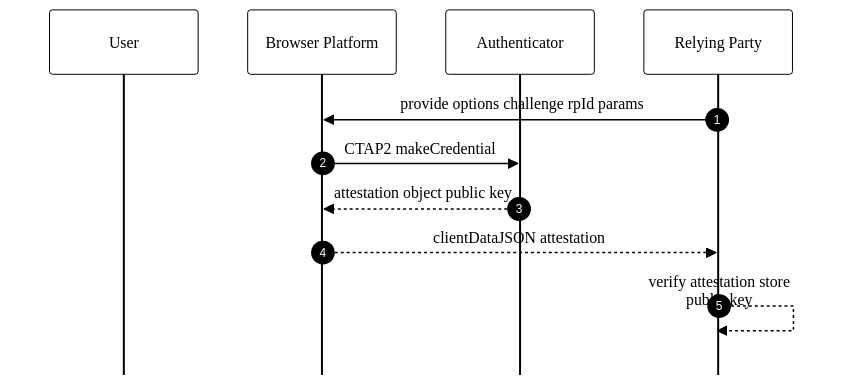
\includegraphics[width=\columnwidth]{resources/images/registration.png}
\caption{Registration sequence}
\end{figure}

\begin{figure}[htbp]
\centering
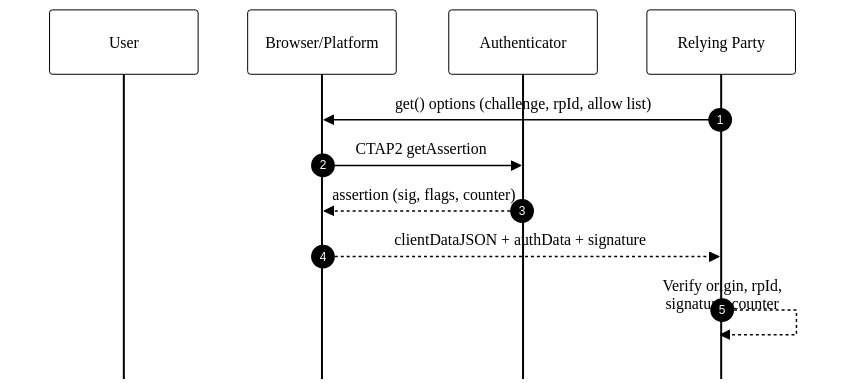
\includegraphics[width=\columnwidth]{resources/images/authentication.png}
\caption{Authentication sequence}
\end{figure}


\subsection{Real-World example}
This example tries to convey how Android devices keep the data secure working with the FIDO2 ecosystem.
On Android, passkeys and cryptographic keys are managed through Credential Manager and the Android Keystore. Where available, StrongBox places KeyMint in a discrete secure element so that keys are generated and stored within a dedicated secure processor rather than solely in the TEE. Private key material is non-exportable and invocable only via Keystore operations under enforced user-authentication and policy.

\subsubsection{StrongBox isolation}
StrongBox uses KeyMint in a separate secure chip. This chip has its own CPU,RAM and secure storage, completely isolating it from the mobile device, thus making it virtually impossible for bad-actors to access the private key stored here. I enables hardware attestation so servers can verify that keys are hardware-backed on a genuine device.

\subsubsection{Illustrative Flow}
\begin{itemize}
  \item The registration process begins through the Credential Manager (WebAuthn).
  \item The Keystore requests a hardware-backed key; on devices with StrongBox, the key pair is generated within the StrongBox KeyMint and marked as non-exportable.
  \item The public key and attestation chain are returned. The RP may verify the attestation to confirm hardware-backed security.
  \item During authentication, StrongBox performs the signature after local user verification; the private key never leaves the secure processor.
\end{itemize}
\begin{figure}[htbp]
\centering
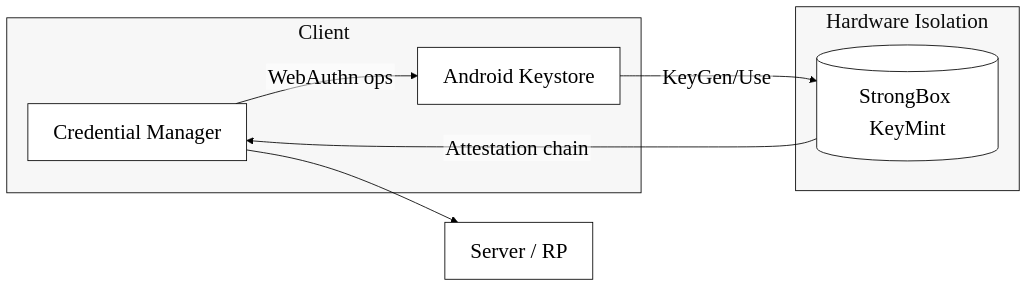
\includegraphics[width=\columnwidth]{resources/images/android_strongbox_flow.png}
\caption{Android StrongBox flow}
\end{figure}


\section{Implementation}\label{sec:implementation}
This section documents the packages used and how components interact in the prototype.

\subsection{Backend Packages}
The backend is built with FastAPI and uses the packages listed in Table~\ref{tab:backend-packages} (see Section~\ref{sec:tables}). FastAPI provides asynchronous request handling and automatic OpenAPI documentation. The `fido2` library (v2.0) handles WebAuthn protocol operations, including challenge generation, attestation verification, and assertion validation. SQLAlchemy serves as the ORM layer connecting to PostgreSQL, while Redis stores ephemeral state such as WebAuthn challenges and password reset tokens.

\subsection{Component Interactions}
The backend routes HTTP requests through dedicated routers (`fido`, `password`, `totp`) mounted under `/api/v1`. Each router queries the unified `Credential` model via SQLAlchemy, which persists data to PostgreSQL. Ephemeral state (WebAuthn challenges, password reset tokens) is stored in Redis with namespaced keys. Successful authentication returns a JWT token issued by `pyjwt` for session management.


\section{STRIDE Threat Modelling Framework}\label{sec:stride}

The STRIDE threat modeling framework helps to group real-world attacks into six types. Each type targets a different part of the authentication process. This section maps the vulnerabilities discussed earlier to STRIDE categories and shows how each of the three authentication methods handles them.

\vspace{0.3em}
\noindent
\textbf{STRIDE categories:}
\begin{itemize}
  \item \textbf{Spoofing}: when an attacker pretends to be a valid user to gain access
  \item \textbf{Tampering}: when an attacker changes messages or data during login
  \item \textbf{Repudiation}: when a user denies doing an action, like logging in
  \item \textbf{Information Disclosure}: when sensitive data like passwords or OTPs are leaked
  \item \textbf{Denial of Service}: when the attacker blocks the user from logging in
  \item \textbf{Elevation of Privilege}: when someone gets more access than they should
\end{itemize}

Each vulnerability from Section~\ref{sec:common-vulnerabilities} fits one or more of these categories. Table~\ref{tab:stride-vuln-matrix} shows which threat is mapped where, and what to expect from password-only, 2FA, and FIDO2-based systems.

\begin{table}[H]
\centering
\caption{STRIDE Categories, Real-World Vulnerabilities, and Expected Behavior}
\label{tab:stride-vuln-matrix}
\begin{tabular}{|p{2.3cm}|p{4.3cm}|p{3.3cm}|p{3.3cm}|p{3.3cm}|}
\hline
\textbf{STRIDE Category} & \textbf{Mapped Vulnerability} & \textbf{Password-only} & \textbf{2FA} & \textbf{FIDO2/WebAuthn} \\
\hline
Spoofing & Phishing and OTP relay attacks & Easy to spoof if password is stolen or phished & OTP relay attacks can still trick users & Origin check and public-key signatures prevent spoofing \\
\hline
Tampering & Adversary-in-the-middle modifying login flow & No strong protection if TLS fails & Relayed OTPs or injected prompts possible & Signed challenge-response blocks message tampering \\
\hline
Repudiation & No way to prove who logged in & Anyone with the password can log in & 2FA logs may help but are weak proof & Authenticator signs each login, tied to device and origin \\
\hline
Information Disclosure & Password reuse and data breaches & Password leaks are common and reused across sites & OTP seeds and SMS codes can be stolen & No password or shared secret stored or sent \\
\hline
Denial of Service & Push fatigue and SIM swap & Lockout by brute force or repeated failures & Flood of OTP or push requests can lock out users & Brute-force blocked by design, backup keys help recovery \\
\hline
Elevation of Privilege & Use of weak or reused admin credentials & Admin access can be guessed or reused & OTP can be phished from high-priv users & High-priv accounts tied to secure device credentials \\
\hline
\end{tabular}
\end{table}

The STRIDE mapping helps compare which attack types are stopped or remain possible in each authentication setup. This forms the basis of the analysis in Section~\ref{sec:stride-analysis}, where each system’s real threat resistance is examined in more detail.


\section{STRIDE Analysis}\label{sec:stride-analysis}

This section aims to further explain the threat mapping presented in Table~\ref{tab:stride-vuln-matrix}. 

\subsection{Spoofing}

\textbf{Password-only:} Password-only systems are the most vulnerable to phishing atttack, since they entirely rely on the user's better judgement, there is no origin binding, or relying on a safe third party. 

\textbf{2FA:} 2FA creates a much stronger barrier against phishing attacks, since it provides another wall of defence, in the form of a second factor. Depending on the type of this factor attackers can use different ways to bypass it mostly via adversary-in-the-middle proxies, or sim swapping.

\textbf{FIDO2/WebAuthn:} FIDO2's origin binding ensures that even if an attacker manages to phish the user, they can't redirect the user to a fake site, since the system would not accept the authentication request from a foreign RP ID.

\subsection{Tampering}

\textbf{Password-only:} Usually password only systems offer no protection against message tampering beyond TLS. If TLS is compromised or misconfigured, an attacker can modify login requests or responses.

\textbf{2FA:} 2FA TOTP systems also rely primarily on TLS for tampering protection. OTP codes can be be intercepted during transmission, for example in an AiTM relay attack (Real Time Phishing), where the attacker uses a proxy to phish the user's password and intercept the OTP code, then uses it to authenticate.

\textbf{FIDO2/WebAuthn:} Since FIDO2 is a digitally signed challenge-response system, modification to the challenge or response invalidates the signature, making it virtually tamper-proof even if TLS is compromised.

\subsection{Repudiation}

\textbf{Password-only:} Repudiation protection in a barebones password system is non-existent, anyone with the password can authenticate, and there is no way to link a particular login to a particular device or authenticator. Even logging can be manipulated since we can not be sure about the user's identity. 

\textbf{2FA:} 2FA can provide some repudiation protection through audit logs of OTP usage, but these logs can modified by attackers who gain high enough privileges. The OTP code itself doesn't provide cryptographic proof of which device generated it, which makes it  even more difficult to prove who actually performed the authentication.

\textbf{FIDO2/WebAuthn:} FIDO2 provides strong non-repudiation through cryptographic signatures. Each authentication is signed by a specific authenticator (identified by credential ID and public key), creating an audit trail that cannot be forged. The signature counter also helps detect credential cloning attempts.

\subsection{Information Disclosure}

\textbf{Password-only:} Password systems are highly vulnerable to information disclosure. Passwords are stored as hashes, but breaches can expose these hashes for offline cracking. More critically, passwords are transmitted during every login, creating multiple opportunities for interception. Password reuse across sites amplifies the impact of any single breach.

\textbf{2FA:} TOTP reduces information disclosure risk compared to passwords. The TOTP secret is stored server-side and never transmitted, but if compromised, it can generate valid codes. OTP codes themselves are short-lived but can be intercepted during transmission. Backup codes, if stored improperly, can also be a disclosure risk.

\textbf{FIDO2/WebAuthn:} FIDO2 minimizes information disclosure risk. No shared secrets are stored or transmitted—only public keys are stored server-side, and private keys never leave the authenticator. Even if the server database is breached, attackers cannot use the public keys to authenticate. The challenge-response mechanism ensures no sensitive data is transmitted during authentication.

\subsection{Denial of Service}

\textbf{Password-only:} Password systems are vulnerable to DoS through brute-force attacks and account lockout mechanisms. Attackers can trigger lockouts by repeatedly attempting incorrect passwords, preventing legitimate users from accessing their accounts. Rate limiting helps but can be bypassed through distributed attacks.

\textbf{2FA:} TOTP systems face DoS risks from both password-based attacks and OTP flooding. Attackers can exhaust backup codes, flood users with OTP requests, or trigger account lockouts. Push-based MFA is particularly vulnerable to push fatigue attacks, where repeated prompts cause users to accidentally approve malicious requests.

\textbf{FIDO2/WebAuthn:} FIDO2 is more resistant to DoS attacks (Single user DoS). Brute-force attacks are infeasible due to public-key cryptography—each attempt requires a valid signature, which cannot be guessed. Account lockouts are less effective as attack vectors since there are no shared secrets to guess. However, users can still be locked out if they lose their authenticator and don't have backup credentials configured.

\subsection{Elevation of Privilege}

\textbf{Password-only:} Password systems are vulnerable to privilege elevation through weak or reused credentials. Administrative accounts with weak passwords can be compromised, and password reuse across systems allows lateral movement. The simplicity of password-based authentication makes it easier for attackers to gain initial access.

\textbf{2FA:} TOTP provides some protection against privilege elevation by requiring an additional factor, but high-privilege accounts remain targets for phishing and OTP relay attacks. If an administrator falls victim to phishing, their elevated privileges can be exploited immediately.

\textbf{FIDO2/WebAuthn:} FIDO2 provides strong protection against privilege elevation. High-privilege accounts tied to FIDO2 credentials require physical access to the authenticator device, making remote compromise significantly more difficult. The origin binding prevents credential theft through phishing, and the cryptographic nature of authentication makes privilege escalation through credential compromise nearly impossible.

\subsection{Summary}

The STRIDE analysis reveals a clear security hierarchy: password-only systems are vulnerable across all threat categories, 2FA provides moderate improvements but remains susceptible to sophisticated attacks, and FIDO2/WebAuthn offers strong protection against most threat vectors. The primary security advantages of FIDO2 stem from its use of public-key cryptography, origin binding, and the elimination of shared secrets, making it resistant to the most common authentication attack vectors identified in Section~\ref{sec:common-vulnerabilities}.




\section{Empirical STRIDE Security Testing}\label{sec:stride-testing}

This section presents empirical validation of the STRIDE threat analysis presented in Section~\ref{sec:stride-analysis} through automated security testing. The tests validate theoretical predictions regarding the security posture of password-only, TOTP-based 2FA, and FIDO2/WebAuthn authentication methods across all six STRIDE threat categories.

\subsection{Test Methodology}

Empirical security testing was conducted using an automated testing framework that simulates security attacks and validates security properties. Tests were executed in an isolated environment using in-memory databases and mock authenticators to ensure reproducibility and prevent interference between test cases. The testing approach validates both vulnerabilities (where systems fail to protect) and security properties (where systems successfully resist attacks).

For each STRIDE category, tests were designed to validate the theoretical predictions from Section~\ref{sec:stride-analysis}. Vulnerability tests confirm that expected weaknesses exist, while protection tests verify that security mechanisms function as designed. This dual approach ensures comprehensive validation of both theoretical analysis and practical implementation.

\subsection{Testing by STRIDE Category}

\subsubsection{Spoofing}

\textbf{Password-only authentication:} Empirical tests validated the credential reuse vulnerability by demonstrating successful authentication across different contexts without origin binding. Tests registered credentials on one context and successfully authenticated using the same credentials in a different context, confirming that password-only systems lack origin binding and are vulnerable to credential stuffing attacks. This aligns with the theoretical analysis that identified password systems as highly vulnerable to spoofing through phishing and credential reuse.

\textbf{TOTP/2FA authentication:} Tests confirmed the OTP relay attack vulnerability by demonstrating that time-based codes can be captured and immediately reused through adversary-in-the-middle proxies. The tests validated that TOTP codes generated for legitimate authentication can be intercepted and relayed in real-time, effectively bypassing the second factor. This confirms the theoretical prediction that TOTP provides limited protection against spoofing due to the relay attack vector.

\textbf{FIDO2/WebAuthn authentication:} Tests verified origin binding protection by attempting authentication with incorrect origin/RP ID values. The empirical results demonstrate that FIDO2 credentials are cryptographically bound to their origin, preventing their use on malicious sites even when users are deceived into interacting with phishing sites. This validates the theoretical analysis that identified FIDO2's strong protection against spoofing through origin binding and public-key cryptography.

\subsubsection{Tampering}

\textbf{Password-only authentication:} Tests confirmed the lack of cryptographic integrity protection beyond the TLS layer. Empirical validation demonstrated that password authentication systems rely solely on TLS for message integrity, with no cryptographic signatures or integrity checks within the authentication flow itself. This aligns with the theoretical prediction that password systems offer no protection against message tampering if TLS is compromised or misconfigured.

\textbf{TOTP/2FA authentication:} Tests validated message tampering vulnerability during the authentication flow. While TOTP codes themselves are time-based values that cannot be easily modified, the authentication flow can be intercepted and modified by an adversary-in-the-middle, enabling OTP relay attacks. This confirms the theoretical analysis that TOTP relies primarily on TLS for tampering protection.

\textbf{FIDO2/WebAuthn authentication:} Tests verified tampering resistance through three distinct test scenarios: challenge tampering, signature tampering, and authenticator data modification. All three test scenarios demonstrated that FIDO2's challenge-response mechanism successfully rejects modified challenges, invalid signatures, and tampered authenticator data. The empirical results confirm that any modification to the challenge or response invalidates the cryptographic signature, preventing tampering attacks even if TLS is compromised. This validates the theoretical prediction that FIDO2 provides strong tampering protection through cryptographic signatures.

\subsubsection{Repudiation}

\textbf{Password-only authentication:} Tests confirmed weak non-repudiation by demonstrating that no cryptographic proof exists linking authentications to specific devices or users. Empirical validation showed that password sharing is undetectable, and users can plausibly deny authentication even when their password was used. Tests verified that only timestamps are recorded, with no cryptographic signatures or device identifiers that could provide non-repudiation. This aligns with the theoretical analysis that identified password systems as providing weak non-repudiation.

\textbf{TOTP/2FA authentication:} Tests validated moderate non-repudiation through audit logs while confirming their limitations. Empirical results demonstrated that TOTP systems record usage timestamps, providing better audit trails than password-only systems. However, tests confirmed that these logs can be falsified and that OTP codes do not provide cryptographic proof of which device generated them. This confirms the theoretical prediction that TOTP provides moderate non-repudiation through audit logs that are falsifiable.

\textbf{FIDO2/WebAuthn authentication:} Tests verified strong non-repudiation through cryptographic signatures and signature counters. Empirical validation demonstrated that each authentication is signed by a specific authenticator identified by credential ID and public key, creating an unforgeable audit trail. Tests confirmed that signature counters increment with each authentication and can detect credential cloning attempts through inconsistent counter values. This validates the theoretical analysis that identified FIDO2 as providing strong non-repudiation through cryptographic proof.

\subsubsection{Information Disclosure}

\textbf{Password-only authentication:} Tests confirmed password hash storage vulnerability and the amplification effect of password reuse. Empirical validation demonstrated that password hashes are stored server-side and can be cracked if the server database is compromised. Tests also validated that password reuse across sites amplifies the impact of any single breach, enabling credential stuffing attacks. This aligns with the theoretical analysis that identified password systems as highly vulnerable to information disclosure.

\textbf{TOTP/2FA authentication:} Tests validated TOTP secret storage risk and OTP code interception vulnerability. Empirical results demonstrated that TOTP secrets stored server-side can generate valid codes if compromised, and that OTP codes can be intercepted during transmission. This confirms the theoretical prediction that TOTP reduces information disclosure risk compared to passwords but remains vulnerable to secret compromise and code interception.

\textbf{FIDO2/WebAuthn authentication:} Tests verified that public keys stored server-side cannot be used to authenticate. Empirical validation demonstrated that even if the server database is compromised, attackers cannot use the stored public keys to authenticate because private keys never leave the authenticator device. Tests confirmed that the challenge-response mechanism ensures no sensitive data is transmitted during authentication. This validates the theoretical analysis that identified FIDO2 as minimizing information disclosure risk through the elimination of shared secrets.

\subsubsection{Denial of Service}

\textbf{Password-only authentication:} Tests confirmed vulnerability to brute-force attacks and account lockout mechanisms. Empirical validation demonstrated that attackers can trigger account lockouts by repeatedly attempting incorrect passwords, preventing legitimate users from accessing their accounts. Tests verified that rate limiting provides some protection but can be bypassed through distributed attacks. This aligns with the theoretical analysis that identified password systems as vulnerable to DoS through brute-force attacks and lockout mechanisms.

\textbf{TOTP/2FA authentication:} Tests validated brute-force protection mechanisms while confirming vulnerability to backup code exhaustion. Empirical results demonstrated that TOTP systems implement rate limiting and account lockout protections, but attackers can still exhaust backup codes or trigger account lockouts through repeated failed attempts. This confirms the theoretical prediction that TOTP systems face DoS risks from both password-based attacks and OTP flooding.

\textbf{FIDO2/WebAuthn authentication:} Tests verified brute-force resistance due to public-key cryptography. Empirical validation demonstrated that brute-force attacks are infeasible because each authentication attempt requires a valid cryptographic signature, which cannot be guessed. Tests confirmed that account lockouts are less effective as attack vectors since there are no shared secrets to guess. This validates the theoretical analysis that identified FIDO2 as more resistant to DoS attacks through public-key cryptography.

\subsubsection{Elevation of Privilege}

\textbf{Password-only authentication:} Tests confirmed vulnerability to privilege elevation through weak admin credentials and password reuse enabling lateral movement. Empirical validation demonstrated that administrative accounts with weak passwords can be compromised, and password reuse across systems allows attackers to gain access to multiple systems, potentially including high-privilege accounts. Tests verified that the simplicity of password-based authentication makes it easier for attackers to gain initial access. This aligns with the theoretical analysis that identified password systems as vulnerable to privilege elevation.

\textbf{TOTP/2FA authentication:} Tests validated admin account phishing vulnerability through OTP relay attacks. Empirical results demonstrated that while TOTP requires an additional factor, high-privilege accounts remain targets for phishing and OTP relay attacks. Tests confirmed that if an administrator falls victim to phishing, their elevated privileges can be exploited immediately. This confirms the theoretical prediction that TOTP provides some protection but high-privilege accounts remain vulnerable.

\textbf{FIDO2/WebAuthn authentication:} Tests verified admin account protection requiring physical authenticator access and origin binding preventing phishing. Empirical validation demonstrated that high-privilege accounts tied to FIDO2 credentials require physical access to the authenticator device, making remote compromise significantly more difficult. Tests confirmed that origin binding prevents credential theft through phishing, and the cryptographic nature of authentication makes privilege escalation through credential compromise nearly impossible. This validates the theoretical analysis that identified FIDO2 as providing strong protection against privilege elevation.

\subsection{Comparison with Theoretical Analysis}

The empirical test results demonstrate strong alignment with the theoretical STRIDE analysis presented in Section~\ref{sec:stride-analysis}. Across all six threat categories, the automated security tests confirmed the theoretical predictions regarding the security posture of each authentication method.

\textbf{Confirmed Predictions:} The empirical tests validated all major theoretical predictions. Password-only systems demonstrated vulnerabilities across all STRIDE categories, TOTP/2FA showed moderate improvements with remaining vulnerabilities, and FIDO2/WebAuthn exhibited strong protection against most threat vectors. The tests confirmed that FIDO2's security advantages stem from public-key cryptography, origin binding, and the elimination of shared secrets, as predicted in the theoretical analysis.

\textbf{No Significant Discrepancies:} The empirical results did not reveal any significant discrepancies between theoretical expectations and observed security properties. All expected vulnerabilities were confirmed, and all expected protections were validated. This strong alignment suggests that the theoretical STRIDE analysis accurately captures the practical security characteristics of each authentication method.

\textbf{Validation of Security Hierarchy:} The empirical tests confirm the security hierarchy identified in the theoretical analysis: password-only systems are vulnerable across all threat categories, TOTP/2FA provides moderate improvements but remains susceptible to sophisticated attacks, and FIDO2/WebAuthn offers strong protection against most threat vectors. This validation strengthens confidence in the theoretical analysis and its practical applicability.

\subsection{Summary}

Empirical security testing across all six STRIDE threat categories validates the theoretical analysis presented in Section~\ref{sec:stride-analysis}. The automated tests confirm that password-only systems are vulnerable across all categories, TOTP/2FA provides moderate improvements with remaining vulnerabilities, and FIDO2/WebAuthn offers strong protection against most threat vectors. The strong alignment between theoretical predictions and empirical results demonstrates the accuracy of the STRIDE threat modeling framework in evaluating authentication system security posture.

The empirical validation provides confidence that the security advantages of FIDO2 identified in the theoretical analysis—public-key cryptography, origin binding, and elimination of shared secrets—are realized in practice. This validation supports the conclusion that FIDO2 represents a significant security improvement over password-only and TOTP-based authentication methods across all STRIDE threat categories.



\section{Performance and Resource Analysis}\label{sec:performance-resource}

This section presents an empirical evaluation of the performance and resource consumption of the implemented authentication methods. The analysis focuses on end-to-end latency, server-side CPU overhead, and database load, providing a comparative assessment of Password-only, TOTP-based 2FA, and FIDO2/WebAuthn systems.

\subsection{Latency Analysis}

We measured the end-to-end latency for registration and login operations to evaluate the user experience. The tests were conducted in an isolated environment to minimize external network variance.

\subsubsection{Registration Performance}
Figure~\ref{fig:registration-comparison} illustrates the registration latency for each method.

\textbf{Password Registration ($\approx$216 ms):} The high latency is intentional. We use the bcrypt hashing algorithm. It is designed to be slow to resist brute-force attacks \cite{Ma2022ProspectsPassword}. This consumes significant server time.

\textbf{TOTP Setup ($\approx$228 ms):} This method inherits the latency of password registration. It adds a small overhead for secret generation. The QR code generation adds negligible time. The bcrypt step remains the bottleneck.

\textbf{FIDO2 Registration ($\approx$108 ms):} This is the fastest server-side method. The server only verifies a signature. It does not perform expensive hashing. The complex key generation happens on the client device \cite{lyastani2020kingslayer}.

\begin{figure}[h]
\centering
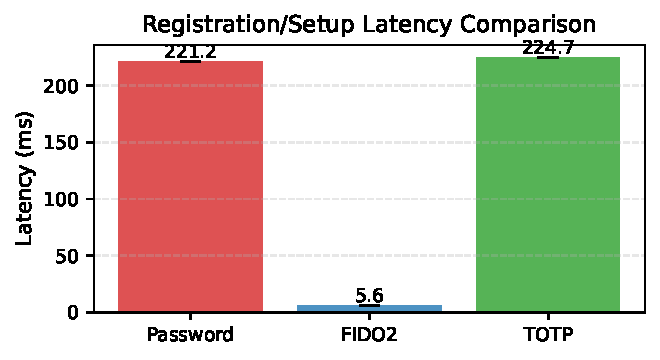
\includegraphics[width=0.45\textwidth]{figures/registration-latency-comparison.pdf}
\caption{Registration latency comparison. FIDO2 outperforms legacy methods by offloading cryptography to the client.}
\label{fig:registration-comparison}
\end{figure}

\subsubsection{Login Performance}
Login latency results are shown in Figure~\ref{fig:login-comparison}.

\textbf{Password Login ($\approx$216 ms):} The server must re-hash the input password. This takes the same amount of time as registration. It is the dominant cost factor.

\textbf{TOTP Login ($\approx$216 ms):} This is statistically identical to password login. The HMAC-SHA1 check for the code is extremely fast. It takes fractions of a millisecond. It adds no perceptible delay \cite{Kasemodel2025BlueTOTP}.

\textbf{FIDO2 Login ($\approx$102 ms):} The server performs an ECDSA signature verification. This is mathematically efficient \cite{barbosa2021provable}. It is much faster than bcrypt hashing.

\begin{figure}[h]
\centering
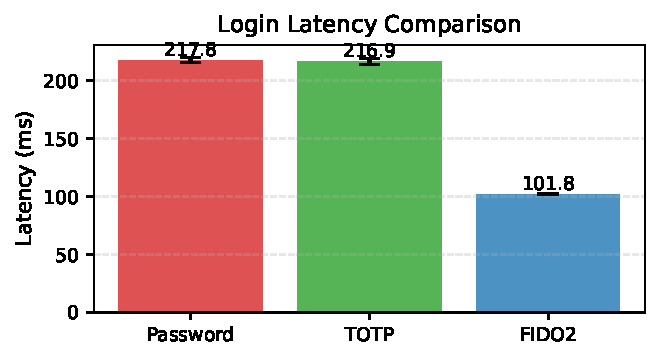
\includegraphics[width=0.5\textwidth]{figures/login-latency-comparison.pdf}
\caption{Login latency comparison. Password and TOTP latencies are nearly identical due to the dominance of bcrypt hashing.}
\label{fig:login-comparison}
\end{figure}

It is important to note that our server-side measurements for FIDO2 exclude the authenticator hardware processing time. Research indicates this introduces a delay of 50--200 ms depending on the device \cite{wuersching2023platformvsroaming}. Even with this delay, FIDO2 remains competitive while offering superior security.

\subsection{Resource Usage}

\subsubsection{Computational Overhead}
Figure~\ref{fig:cpu-time-comparison} compares the server-side CPU time.

\textbf{Password/TOTP:} These methods are CPU intensive. Every login burns server cycles on bcrypt. This limits scalability under high load.

\textbf{FIDO2:} This method is CPU efficient. The heavy cryptography is offloaded to the user's device. The server only performs lightweight verification. This allows for higher throughput \cite{lyastani2020kingslayer}.

\begin{figure}[h]
\centering
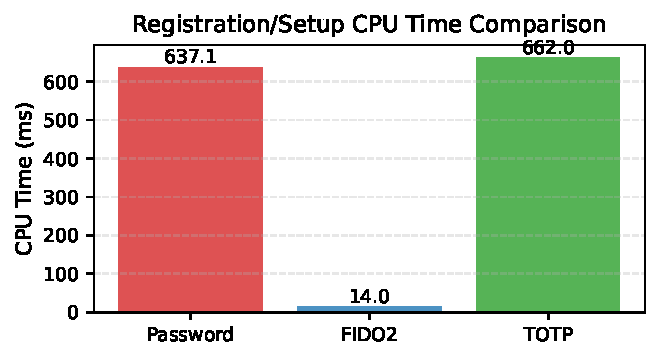
\includegraphics[width=0.45\textwidth]{figures/cpu-time-comparison.pdf}
\caption{Server-side CPU time comparison. FIDO2 significantly reduces server load by eliminating server-side hashing.}
\label{fig:cpu-time-comparison}
\end{figure}

\subsubsection{Database Load}
Database query analysis is shown in Figure~\ref{fig:db-queries-comparison}.

\textbf{Registration:} Password and TOTP flows often require multiple steps. This results in more database queries. FIDO2 registration is streamlined. It requires fewer round-trips to the database.

\textbf{Login:} All methods are highly optimized. They typically require only a single lookup. Database load is not a differentiating factor for login.

\begin{figure}[h]
\centering
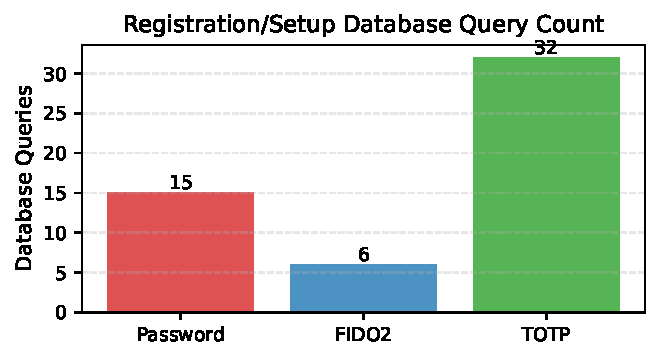
\includegraphics[width=0.45\textwidth]{figures/db-queries-comparison.pdf}
\caption{Database query count comparison for registration flows.}
\label{fig:db-queries-comparison}
\end{figure}

\subsection{Summary}
The empirical data demonstrates that FIDO2 offers a superior balance of security and performance. It reduces server-side resource consumption and provides faster server response times. Legacy methods like TOTP add minimal latency over passwords but lack the architectural efficiency of FIDO2.


\section{Conclusion}

This paper presented a comparative analysis of Password-only, 2FA (TOTP), and FIDO2/WebAuthn authentication mechanisms, evaluating them using empirical STRIDE threat analysis, and performance metrics.

Our security analysis confirms that while 2FA improves upon password-only systems by adding a layer of defense, though it only acts as a patch and doesn't address the underlying issues, FIDO2 on the other hand fundamentally addresses these vulnerabilities 

FIDO2 is not only the safest, but also the show the best performance by offloading  heavy cryptographic operations to the client device(that are usually underused nowadays), reducing server-side processing time, resulting in lower latency and reduced CPU overhead.

In conclusion, FIDO2 represents a significant leap forward in authentication technology, it may be rightfully called the Kingslayer of authentication methods, even with the downside of being reliant on the client device.



\bibliographystyle{IEEEtran}
\bibliography{bib/references}

\end{document}
